3\documentclass[11pt,letterpaper]{article}
\usepackage[latin1]{inputenc}
\usepackage{amsmath}
\usepackage{amsfonts}
\usepackage{amssymb}
\usepackage{graphicx}
\usepackage{capt-of}

\setlength{\parskip}{1pc}
\setlength{\parindent}{0pt}
\setlength{\topmargin}{-3pc}
\setlength{\textheight}{9.0in}
\setlength{\oddsidemargin}{0pc}
\setlength{\evensidemargin}{0pc}
\setlength{\textwidth}{6.5in}

\title{6.170 Assignment 5 Documentation}
\author{Dina Betser}


\begin{document}
\maketitle

\section{Models}
\subsection{Object Models}
The object model for the problem domain is included in the figure below. The problem domain object model demonstrates the system that must be built. 

Within the application, \texttt{User}s have a set of \texttt{Note}s. Every user has a \texttt{UserId}, \texttt{Password}, and \texttt{Username}.  Every Note has a \texttt{NoteId}, \texttt{Position}, and some type of \texttt{Content}. For this application, every Note only contains an instance of \texttt{TextContent}, though an extension could allow a Note to contain other types of Content, such as an image.
\begin{center}
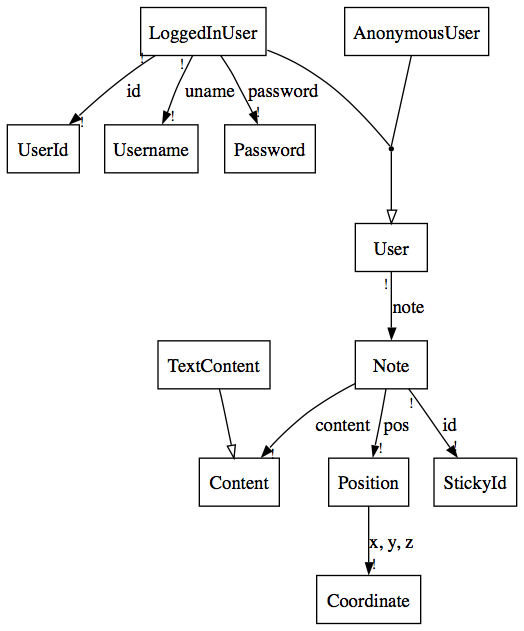
\includegraphics[width=5in]{dot/obmod.png}
\label{fig:ob1} 
\end{center}

\subsection{State Machines}
The following state machine describes how the state of the application changes as a user uses the sticky note application. The user is either logged in or out, and can only add, edit, or delete stickies from the logged-in state.
\begin{center}
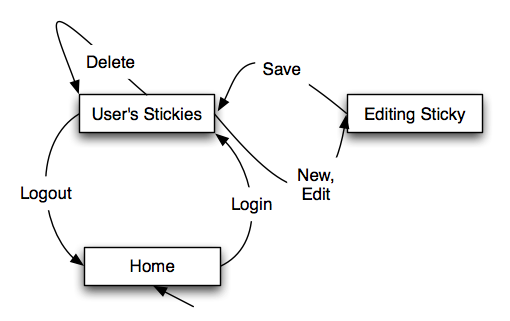
\includegraphics[width=7in]{dot/statediagram.png}
\label{fig:sm1} 
\end{center}

\section{Design Notes}
\subsection{Key Challenges}
\begin{itemize}
\item Does a user need to be logged in to create stickies? If not, should all ``current stickies'' be saved upon login?\\
At first, I thought it would make the most sense to allow users to create stickies without being logged in. Then, upon login, all the current notes would be saved persistently for that user. This scheme was more complex than the final decision, which was to only allow users to edit stickies upon login.
\item Editing notes on the fly or using a popup dialog.\\
It would have been possible to pop up a dialog box whenever a user wanted to edit or add a new sticky. However, this is less usable, as it covers the window and prevents the user from interacting with the rest of the interface. Therefore, I decided to open up a textarea that allowed for editing but didn't prevent interaction with the rest of the functionalities of the application.
\item Status of server -- should it be stateless?\\
In class we discussed that the paradigm for servers is for them to be stateless. For this reason, I refrained from storing a map of logged-in statuses for users in the server and let Flask deal with session management on a per-request basis.
\end{itemize}

\subsection{Issues Arising}
\begin{itemize}
\item Implementing login by using the flask-login module. \\
Flask-login proved to be fairly hard to use correctly. Adding a registration capability is outside the scope of flask-login, and combining registration with authentication was not trivial. It proved much simpler and clearer to use session variables to represent a user's login state.
\item Stickies ``jump'' upon save.\\
For some reason, after stickies are dragged, when the new position is saved and then reloaded, the sticky often ``jumps'' to the left and downwards. I think this is because I am not taking into account the size of the sticky itself when saving its position. Time pressures of this project prevented debugging this, but fortunately, it does not detract much from the user's ability to move stickies at will.
\end{itemize}

\subsection{Critique}
This project implemented separation of concerns by using the MVC design pattern. Each module created had a clear specification and purpose, so the code itself was organized fairly well. All controller code was stored in \texttt{stickies.js}, while all model objects were stored in \texttt{stickies\_model.py}. These objects followed directly from the object model in this document.

The interface is not particularly visually appealing, and the stickies are somewhat garishly yellow, but it meets the specifications. If I had more time, I would improve the CSS styling of the interface to make it more aesthetically pleasing. I would also prefer to fix the issue where stickies ``jump'' upon save.

I learned a lot about building a web application from the ground-up from doing this project and it served as a good way to get acquainted with shelve, Flask, and remind myself about using GET and POST requests, and HTTP status codes. I now have a new favorite HTTP Status (401 -- see figure below)!

\begin{center}

\includegraphics[width=4in]{dot/401.jpg}
\label{fig:401} 
\end{center}

\section{Specification}
\subsection{Overview}
This application is a web application written using HTML/CSS/JavaScript on the client-side, and the Python Flask framework (with shelve for persistent storage) on the server side.

The application allows users to store and edit stickies containing text, and to access these stickies from any machine using their login information.

\subsection{Key Features}
The key features of this implementation of the 6.170 Network Stickies implementation are:
\begin{itemize}
\item Users can access their stickies from any browser. Login information is stored in the backend so the scheme is tolerant of browser failures.
\item Smooth dragging allows users to arrange stickies anywhere in the field of view simply by dragging the mouse. The position of stickies on the page is stored across sessions.
\item Features on the page are visible when applicable, and hidden when not. For instance, when a user clicks ``Edit'' on a sticky, the editing box appears for the user to edit. There are no popups or alerts, which generally hinder visibility.
\item An external script \texttt{init\_db.py} allows for refreshing the database for testing purposes.
\item The size of the sticky is dependent on the amount of text entered, making the application more flexible.
\item Passwords are not stored in the backend in cleartext, making the application more secure.
\end{itemize}

\subsection{User Manual}
The running application can be accessed at https://courses.csail.mit.edu/6.170/sp12/students/dbetser/
assignment4/index.fcgi .

A new user should be registered by clicking on the ``Register'' link, and filling in the desired name and password. Thereafter, the user can login with that same name and password to access stickies.

New stickies are added via the ``Add Sticky'' button. The text of the sticky should be entered into the box that appears, and submitted by clicking the box called ``Submit''.

Existing stickies are edited by clicking the ``Edit'' button on the sticky, updating the text that appears near the top of the window, and clicking the Update button.

Stickies are deleted by clicking the ``Delete'' button for that sticky.

To move a sticky, merely click on it and drag it to its new position. Stickies can be stacked vertically as well.

No functionalities can be accessed without logging in first.

\section{Implementation}

\subsection{Module Dependency Diagram}
This code's modules can be seen in the context of the Model-View-Controller framework, which is roughly related to how the files were defined. The \texttt{stickies.js} file contains the Controller, while \texttt{stickies\_model.py} contains the model objects, which includes the objects defined in the object model above. Concerns are separated cleanly in that no code in the model touches anything in the user interface. The model is further stored in a database where user information is kept persistently. The \texttt{main.py} serves to wrap the database and return views to the client upon requests from the browser. The Controller consists of functions that handle events in the UI, such as the form submission and click handling functions. The controller is responsible for sending POST requests to the Flask application server.

This code is written using the jQuery and jQuery UI libraries for DOM handling and convenience functions. The figure below shows the module dependency diagram.

\begin{center}
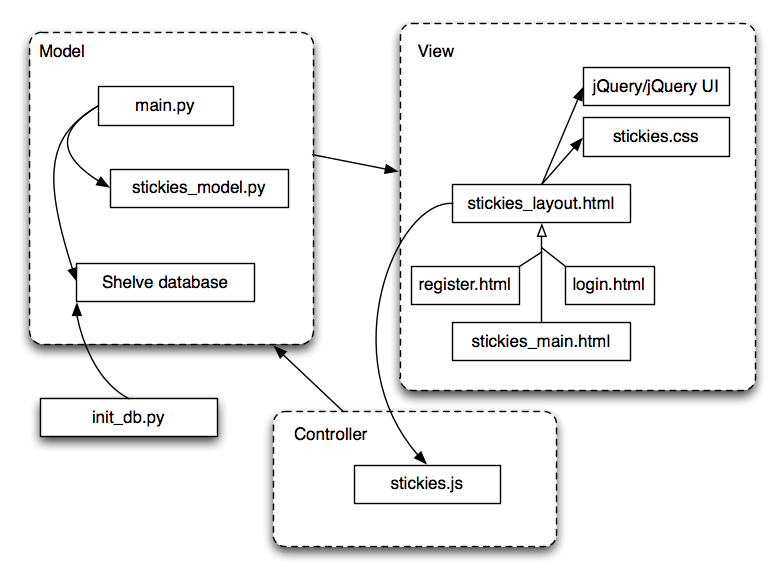
\includegraphics[width=400pt]{dot/moddep.png}
\label{fig:ob2} 
\end{center}
\subsection{Code Notes}
I needed to set the position of a sticky based on the position stored in the database, which violated separation of concerns to some extent because CSS was stored in the HTML tag for each sticky.

One interesting construct that appears in my JavaScript code has to do with using AJAX for adding stickies. At first, I was using form submission for adding stickies. However, the assignment prescribed that AJAX was used for user interaction, so I modified the JavaScript controller code to use POST requests for sticky interaction. However, to update the view upon return of the POST requests, I needed to call:
\begin{verbatim}
window.location.replace($SCRIPT_ROOT);
\end{verbatim}
which seems to me is not ideal. I'm interested in hearing ideas for how to avoid this in the future.

\section{Testing}

\subsection{Test Plan}
To test the application, the HTML was validated to ensure standards compliance. Pychecker was run to remove style issues.

A test suite was developed for the application using Python unit testing. The tests in the file \texttt{stickies\_test.py} cover the functionalities of registration, login, adding, editing, and deleting stickies, and logout. They also ensure that a 401 status is returned when a non-logged-in user tries to access a page requiring login.

In addition, manual testing was done to ensure that the application functioned as specified.

\subsection{Rationale and Conclusions}
This project fulfills the requirements of the assignment. The application runs as desired, is well-commented, and demonstrates separation of concerns.

Many of the design decisions implemented made the interface easier and cleaner to use, which improved the overall user experience. There is more work to be done to improve the appearance of the application, but overall it served as a good learning experience for using the Python Flask framework.

\end{document}

